\section{Tests of Parameters Performance}
%\begin{enumerate}
%\item Introduction to the section. What do we want and why. First we want to test A and the X. At last we want to test the complete system.
%\item Introduce how we will compare the tests and how we measure the quality -- Mean Squared Error (MSE).
%\item Subsection with the error measure
%\item Subsection with a introduction to the data sets -- AR and Toy Example data sets.
%\item Subsection with the performing of tests
%	\begin{itemize}
%	\item Talk about the choice for a initial A in the Cov-DL when D is under-complete. Random uniform distribution? or a Gaussian distribution. Show the errors of the real A and estimated A.
%	\item With the choice for A we now tests the choice for the number of segmentation in Cov-DL.
%	\item Test X with the found A. Make a comparison of the error for X and A in one plot.
%	\end{itemize}
%\end{enumerate}
With the implemented algorithms -- Cov-DL and M-SBL -- the purpose is now to investigate the performance of each algorithm. The performance will be measure by a error measure -- the mean square error (MSE) -- this will be presented in the next section. To make a realistic conclusion on the performance values achieved from the MSE the performance of the algorithms will be compared to the MSE value of the performance of the algorithm with a known mixing matrix $\mathbf{A}$. All the tests will be done one the estimated matrices but for the comparison of these error measurement the true mixing matrix will be used. As the true $\mathbf{A}$ is used we can not compared the performance of Cov-DL but only M-SBL as this used the mixing matrix $\mathbf{A}$ as inputs. The Cov-DL algorithm will instead be tested for different choice of parameters, the initial $\mathbf{A}_{\text{ini}}$ using in the Cov-DL for the optimisation part of finding the matrix $\mathbf{D}$, and the segmentations in Cov-DL as well.
Each test will be looking at one parameter of the algorithm where it is the performance of that parameter there will be measured.

The goal with all these tests is make the best choice for each parameters, to achieve lowest error, such that when the baseline algorithm is used on realistic data set, the EEG measurements, the parameters as been chosen with the best performance in mind -- leading to the best scenario of finding the true mixing matrix and source matrix from EEG measurements.

First at all, we will run a test, with random setting, to see how the error margin is for both algorithms.

\subsection{Error}
To evaluate performance of the algorithms we will be looking at the differences between the real and estimated matrices, mixing matrix $\mathbf{A}$ and source matrix $\mathbf{X}$.
For this task a mean squared error (MSE) method has been chosen. 
The MSE method measure the average squared difference between some estimated value and the actual value. 
%The MSE has the property of always being positive because of the randomness introduced in the method.
The MSE can be written as
\begin{align*}
\text{MSE} = \frac{1}{T} \sum_{i=1}^T (G_i - \hat{G}_i)^2,  
\end{align*}
with $T = \{M, k\}$ the numbers of rows of $\mathbf{A}$ or $\mathbf{X}$, $G_i = \{ \mathbf{A}_i, \mathbf{X}_i\}$ is a measurement row of the actual matrix and $\hat{G}_i = \{\hat{\mathbf{A}}_i,\hat{\mathbf{X}}_i\}$ is an estimated row of the estimated matrix.
The MSE is viewed as a measure of the quality of an estimator, in this case of how M-SBL and Cov-DL perform. 
For a large MSE value the estimated matrix/values are dispersed widely around its mean while for a small MSE value the estimated matrix/values is closely dispersed around the mean. 
Usually, a small MSE value indicate a good estimator but the value cannot be to small as this would indicate that the data has been overfitted \todo{Vi skal lige finde en god kilde som siger dette}. 
Therefore, a good MSE and therefore a good performance would be depending on how the data is scattered as widely scattered data may lead to a MSE value not close to zero but it would still be the a good measure for the estimator.

\subsection{Simulation of Data Sets}\label{sec:dataset}
For the test of the performance of the algorithms some simulated data sets will be used as we then know the real mixing matrix and source matrix which will be using when measuring the performance with MSE.

Two data sets has been made, one which is just a simple data set with simple measurement, and one which is more random and fluctuated -- more like real EEG measurements.

\subsubsection{Simple Data Set}
The simple data set is a date set which do not represent realistic data, EEG measurements, but is only used to confirm that the two algorithm works and to test the performance.
The simple data set is constructed from four different signals representing the sources of the source matrix $\mathbf{X}$: 
\begin{itemize}
\item[-] a sinus signal $\sin(2t)$
\item[-] a sinus signal $\sin(4t)$
\item[-] a sawtooth signal with period $2 \pi t$
\item[-] a sign signal of $\sin(3t)$
\end{itemize}
with $t$ being a time index defined in the interval $[0,10]$ with $L$ samples. Each of the four signal are randomly drawn and used to construct a source matrix $\mathbf{X}$ of size $k \times L$. Therefore some of the signals may occur two or more time as sources.
The mixing matrix $\mathbf{A}$ of size $M \times k$ is randomly generated from a Gaussian distribution. Its rows are then normalised. 
By multiplying the source matrix and the mixing matrix the measurement matrix $\mathbf{Y}$ is achieved.
The simple data set then consist of $\{ \mathbf{Y}, \mathbf{X}, \mathbf{A} \}$ which are the true values of the MMV model.

An illustration of the measurement matrix $\mathbf{Y}$ from the simple data set can be seen in figure \ref{fig:mix}. The data set is constructed for $M = 3$, $k = 4$ and $L = 1000$.
\begin{figure}[H]
\centering
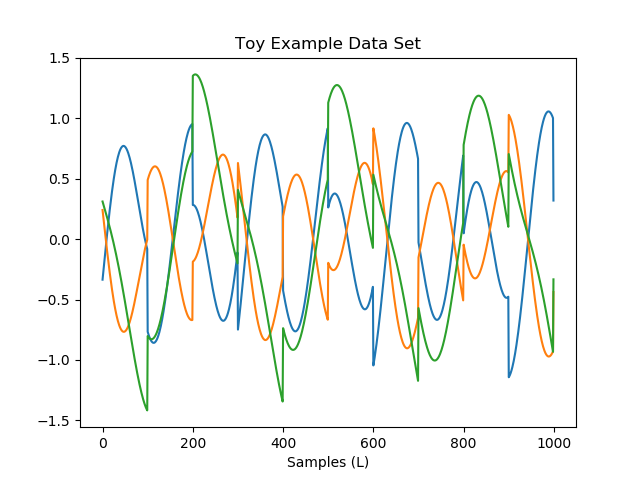
\includegraphics[scale=0.5]{figures/chapter6/Mix_Data_m3_n4_k4_L1000.png}
\caption{This is a visualization of the measurement matrix $\mathbf{Y}$ from the simple data set for $M = 3$, $k=4$ and $L=1000$. As $k = 4$ there are four signals representing the measurement matrix $\mathbf{Y}$.}
\label{fig:mix}
\end{figure}
\noindent

\subsubsection{Autoregressive Data Set}
The second data set illustrate a more realistic data set.
The data set is constructed from four different autoregressive processes representing the sources of the source matrix $\mathbf{X}$ \todo{Skal lige finde en god måde at skrive dem ind på}: 
\begin{itemize}
\item[-] $\mathbf{x}^{t} = \mathbf{a1}^{t-1} \cdot \mathbf{x}^{t-1} + \mathbf{a1}^{t-2} \cdot \mathbf{x}^{t-2} + \mathbf{w1}_t$
\item[-] $\mathbf{x}^{t+1} = \mathbf{a2}_t \cdot \mathbf{x}_{t-1} + \mathbf{a}_t \cdot \mathbf{x}_t + \mathbf{w}_t$
\item[-] $\mathbf{x}_{t+1} = \mathbf{a}_t \cdot \mathbf{x}_{t-2} + \mathbf{a}_t \cdot \mathbf{x}_t + + \mathbf{a}_t \cdot \mathbf{x}_{t-1} \mathbf{w}_t$
\item[-] $\mathbf{x}_{t+1} = \mathbf{a}_t \cdot \mathbf{x}_t + \mathbf{a}_t \cdot \mathbf{x}_{t-3} + \mathbf{w}_t$
\end{itemize}
Each of the four autoregressive processes are randomly drawn and used to construct a source matrix $\mathbf{X}$ of size $k \times L$. 
The mixing matrix $\mathbf{A}$ of size $M \times k$ is randomly generated as the same way as the mixing matrix from the simple data set, from a Gaussian distribution. 
By multiplying the source matrix and the mixing matrix the measurement matrix $\mathbf{Y}$ is achieved.
The autoregressive data set then consist of $\{ \mathbf{Y}, \mathbf{X}, \mathbf{A} \}$ which are the true values of the MMV model.

An illustration of the autoregressive data set can be seen in figure \ref{fig:AR}. The data set is constructed for $M = 3$, $k = 4$ and $L = 1000$.
\begin{figure}[H]
\centering
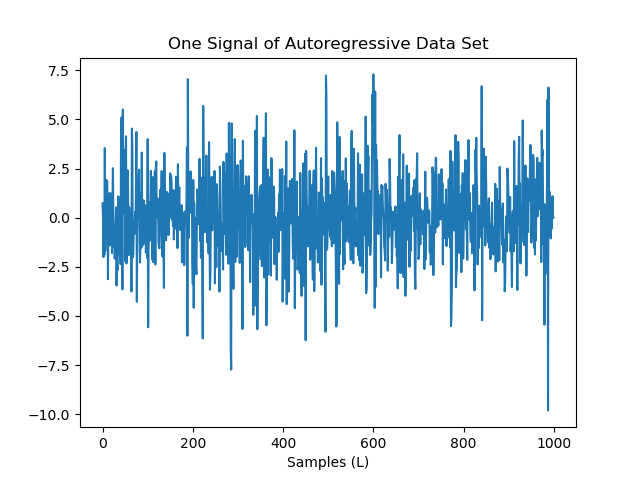
\includegraphics[scale=0.5]{figures/chapter6/AR_Data_m3_n4_k4_L1000.png}
\caption{This is a visualization of the first row of the measurement matrix $\mathbf{Y}$ from the autoregressive data set for $M = 3$, $k=4$ and $L=1000$.}
\label{fig:AR}
\end{figure}
\noindent
As $k = 4$ there are four signals representing the measurement matrix $\mathbf{Y}$ but only one signal is visible in figure \ref{fig:AR}. By visualizing all signals at once as in \ref{fig:mix} it would be difficult to see all the signal apart each other.

\subsection{Tests}
Before any testing of the performance of the algorithms we will test if the algorithms give us a reasonable result. The Cov-DL and M-SBL has been tested with the simple data to see if the algorithms give us a results and how the performance of M-SBL differs when using an estimated mixing matrix and the true mixing matrix.

In the following figure we see the recovered sources aligned with the real source of a system with $M = 3$ and $k = 4$ for $L = 100$ -- a small system.
\begin{figure}[H]
    \begin{minipage}{0.5\linewidth}
    	\centering
        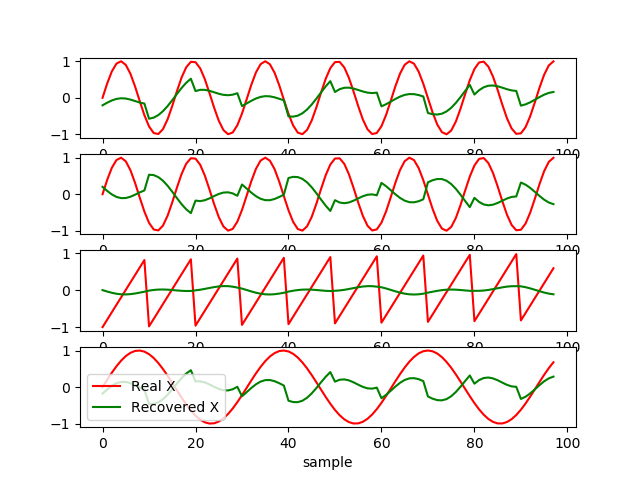
\includegraphics[scale=0.5]{figures/chapter6/test_of_algo_mix_data.png}
		\caption{The $k$ recovered sources from M-SBL with the estimated mixing matrix $\mathbf{A}$.}
		\label{fig:test_toy}
    \end{minipage} 
    ~\hfill~
    \begin{minipage}{0.5\linewidth}
    	\centering
        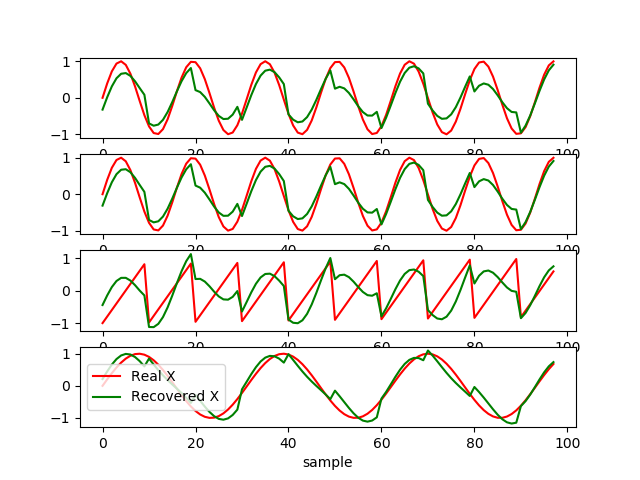
\includegraphics[scale=0.5]{figures/chapter6/test_of_algo_mix_data_realA.png}
		\caption{The $k$ recovered sources from M-SBL with the real mixing matrix $\mathbf{A}$}
		\label{fig:test_toy_realA}
    \end{minipage}
\end{figure}
\noindent
From figure \ref{fig:test_toy} we see that four signal (our sources) has been recovered which is identical with the number of sources in the simple data set. Furthermore, we see that the estimation of the sources are not identical with the real sources but follow some patterns of the real sources. For example source one and two in \ref{fig:test_toy} increase and decrease at the same samples but not with the same amplitude as the estimated sources are more constant like than the sinus signals which is the real sources. Source three look more like a sinus signal than a sawtooth signal. The last source do not look like the sinus signal.
In figure \ref{fig:test_toy_realA} the real mixing matrix is used when estimating the source matrix with M-SBL. Here we see that sources look more like the real sources expect source three.
To compare the two estimation of the source matrix $\mathbf{X}$ the MSE has been applied:
\begin{table}[H]
\centering
\begin{tabular}{|c|c|c|}
\hline
         & Estimated $\mathbf{A}$ & Real $\mathbf{A}$ \\ \hline
MSE of $\mathbf{A}$ & 2.16 & $\times$ \\ 
\hline 
MSE of $\mathbf{X}$ & 0.49 & 0.14 \\ 
\hline
\end{tabular} 
\caption{MSE values of the mixing matrix $\mathbf{A}$ and source matrix $\mathbf{X}$ from the Simple Data Set}
\label{tab:test}
\end{table}
\noindent
From \ref{tab:test} we see that the estimated source matrix has low MSE value. This is due to the low value in $\mathbf{X}$ that the error also is small. But we see a different between the used of a estimated mixing matrix and the real mixing matrix.

\subsubsection{Initial A in Cov-DL}
For the Cov-DL algorithm when estimating the mixing matrix $\mathbf{A}$ a matrix $\mathbf{D}$ is used in the recovering process. For a over-determined system \ref{sec:over_det} $\mathbf{D}$ is found from an optimisation problem \eqref{eq:Cov_DL2} created with use of principal component analysis. To solve the optimization problem and finding $\mathbf{D}$ an initial $\mathbf{A}_{\text{ini}}$ is used as a starting point in the optimization process. The choice of this initial $\mathbf{A}_{\text{ini}}$ will affect how the good an estimate our recovered mixing matrix $\hat{\mathbf{A}}$ is.

In this section we will be testing three different choice for $\mathbf{A}_{\text{ini}}$:
\begin{itemize}
\item[-] A matrix $\mathbf{A1}$ drawn from a continuous uniform distribution in the half-open interval $[0.0, 1.0)$
\item[-] A matrix $\mathbf{A2}$ drawn from a uniform distribution in the half-open interval $[-1.0, 1.0)$
\item[-] A matrix $\mathbf{A3}$ drawn from a Gaussian distribution with mean 0 and variance 1
\end{itemize}
The test of different initial $\mathbf{A}_{\text{ini}}$ will be performed on the both data sets presented in \ref{sec:dataset}. The goal with this test is to find the best initial $\mathbf{A}_{\text{ini}}$. The results are based on MSE of both the Cov-DL with $\mathbf{A}_{\text{ini}}$ and the M-SBL which used the recovered $\mathbf{A}$ as input and therefore also is affect by the choice of $\mathbf{A}_{\text{ini}}$.

When it comes to finding the best initial $\mathbf{A}_{\text{ini}}$ it must be taken into account that the realistic data set -- the EEG measurements -- are more random distributed and have higher amplitude than our simple data set so we are more likely to look at the result for the autoregressive data set as it more resembling the EEG measurements. This lead to that the choice for $\mathbf{A}_{\text{ini}}$ may have a higher error in the simple data set than the autoregressive data set.

For the test we are looking at a system of size $M = 8$, $k = 16$ and $L = 1000$. Furthermore, for the Cov-DL the data has been divided in segments of 10 samples leading to 100 segments.
\begin{figure}[H]
\centering
    \begin{minipage}[t]{.45\textwidth}
        \centering
		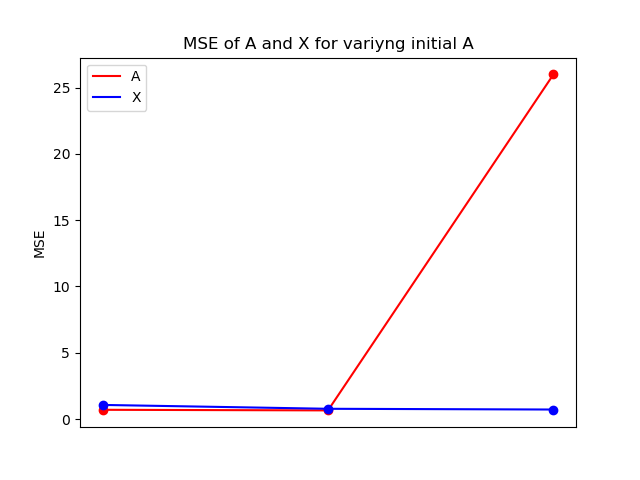
\includegraphics[scale=0.5]{figures/chapter6/Mix_Error_initial_A_m8_k16_L1000.png}
		\subcaption{Simple Data Set - Estimated A}
    \end{minipage} 
    \hfill
    \begin{minipage}[t]{.45\textwidth}
        \centering
		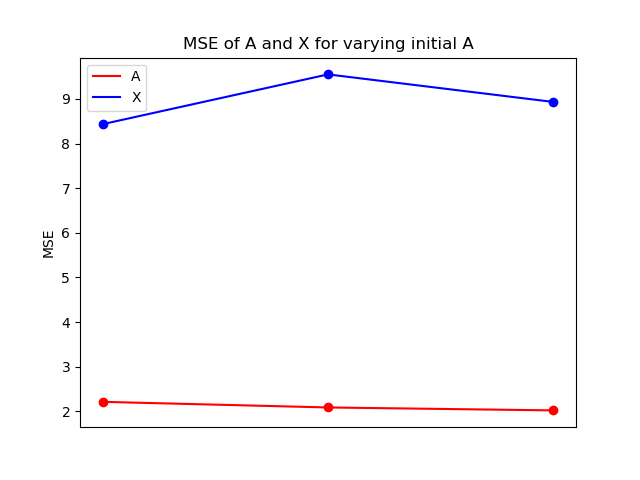
\includegraphics[scale=0.5]{figures/chapter6/AR_Error_initial_A_m8_k16_L1000.png}
		\subcaption{Autoregressive Data Set - Estimated A}
    \end{minipage}
    \begin{minipage}[t]{.45\textwidth}
        \centering
		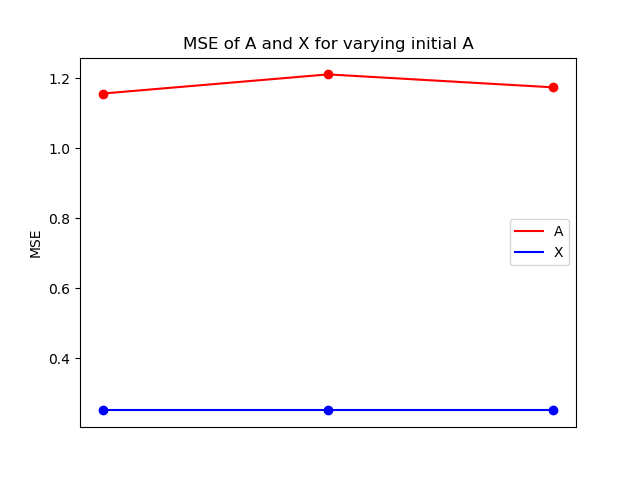
\includegraphics[scale=0.5]{figures/chapter6/Mix_Error_initial_A_m8_k16_L1000_RealA.png}
		\subcaption{Simple Data Set - Real A}
    \end{minipage} 
    \hfill
    \begin{minipage}[t]{.45\textwidth}
        \centering
		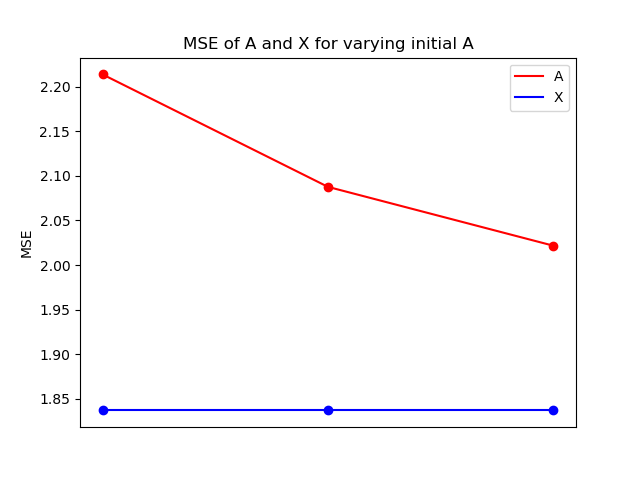
\includegraphics[scale=0.5]{figures/chapter6/AR_Error_initial_A_m8_k16_L1000_RealA.png}
		\subcaption{Autoregressive Data Set - Real A}
    \end{minipage}
\caption{}
\label{fig:initialA}
\end{figure}
\noindent
The MSE values of each tests -- estimated and real mixing matrix $\mathbf{A}$ -- can be seen in table \ref{tab:iniA}. For the real mixing matrix the MSE values of source matrix $\mathbf{X}$ are identical because the real mixing matrix is not influenced by the three different initial $\mathbf{A}_{\text{ini}}$.
\begin{table}[H]
\begin{minipage}{.5\linewidth}
\centering
\begin{tabular}{|c|c|c|c|}
\hline 
 & $\mathbf{A1}$ & $\mathbf{A2}$ & $\mathbf{A3}$ \\ 
\hline 
MSE of $\mathbf{A}$ & 1.16 & 1.21 & 1.17 \\ 
\hline 
MSE of $\mathbf{X}$ & 0.69 & 0.66 & 0.81 \\ 
\hline 
\end{tabular} 
\subcaption{Simple Data Set - estimated $\mathbf{A}$}
\end{minipage}
\begin{minipage}{.5\linewidth}
\centering
\begin{tabular}{|c|c|c|c|}
\hline
 & $\mathbf{A1}$ & $\mathbf{A2}$ & $\mathbf{A3}$ \\ 
\hline 
MSE of $\mathbf{A}$ & 2.21 & 2.09 & 2.02 \\ 
\hline 
MSE of $\mathbf{X}$ & 8.43 & 9.55 & 8.93 \\ 
\hline
\end{tabular} 
\subcaption{Autoregressive Data Set - estimated $\mathbf{A}$}
\end{minipage}
\begin{minipage}{.5\linewidth}
\centering
\begin{tabular}{|c|c|c|c|}
\hline 
 & $\mathbf{A1}$ & $\mathbf{A2}$ & $\mathbf{A3}$ \\ 
\hline 
MSE of $\mathbf{A}$ & $\times$ & $\times$ & $\times$ \\ 
\hline 
MSE of $\mathbf{X}$ & 0.25 & 0.25 & 0.25 \\ 
\hline 
\end{tabular} 
\subcaption{Simple Data Set - real $\mathbf{A}$}
\end{minipage}
\begin{minipage}{.5\linewidth}
\centering
\begin{tabular}{|c|c|c|c|}
\hline
 & $\mathbf{A1}$ & $\mathbf{A2}$ & $\mathbf{A3}$ \\ 
\hline 
MSE of $\mathbf{A}$ & $\times$ & $\times$ & $\times$ \\ 
\hline 
MSE of $\mathbf{X}$ & 1.84 & 1.84 & 1.84 \\ 
\hline
\end{tabular} 
\subcaption{Autoregressive Data Set - real $\mathbf{A}$}
\end{minipage}
\caption{(a) This are the MSE values achieve from the simple data set and (b) is the MSE values achieved from the autoregressive data set.}
\label{tab:iniA}
\end{table}
\noindent
From \ref{tab:iniA} we see that the MSE values for our estimated mixing matrix $\mathbf{A}$ are overall small compared to both data sets. However, if we look at the results for the source matrix there are a big different from the simple data set and the autoregressive data set and comparing it to the results with the real mixing matrix. 
As the autoregressive data set have a higher amplitude in the data than the simple data set, the error will become larger. 

If we look at the initial $\mathbf{A}_{\text{ini}}$ drawn from the Gaussian distribution we have a small error for the mixing matrix in the autoregressive data set while the error from the simple data set also is low. The error for source matrix is the highest value for the simple data set but comes second in the autoregressive data set. As we want to take into account that the autoregressive data set resemble the EEG measurement most we conclude that the initial $\mathbf{A}_{\text{ini}}$ from the Gaussian distribution would be the best choice in Cov-DL.

\subsubsection{Segmentation in Cov-DL}
\begin{figure}[H]
\centering
    \begin{minipage}[t]{.45\textwidth}
        \centering
		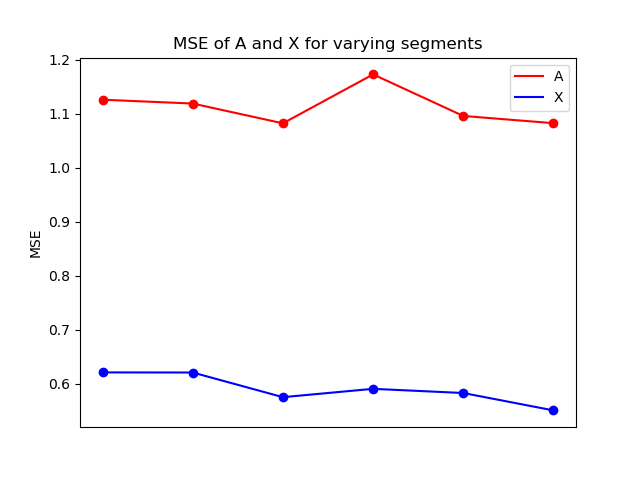
\includegraphics[scale=0.5]{figures/chapter6/Mix_Error_vary_covseg_m8_k16_L1000}
		\subcaption{Simple Data Set - Estimated A}
    \end{minipage} 
    \hfill
    \begin{minipage}[t]{.45\textwidth}
        \centering
		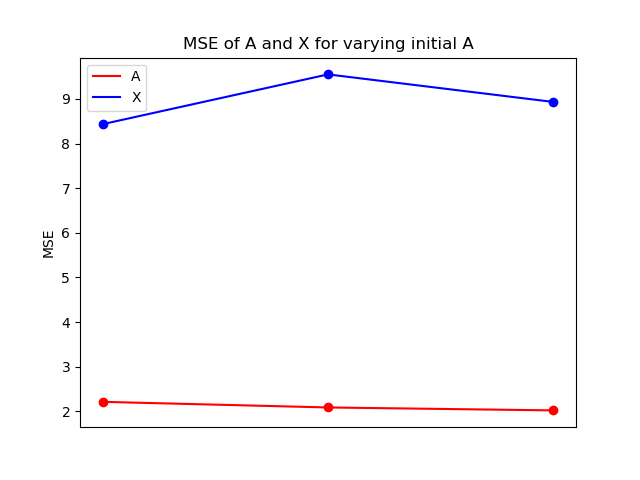
\includegraphics[scale=0.5]{figures/chapter6/AR_Error_initial_A_m8_k16_L1000.png}
		\subcaption{Autoregressive Data Set - Estimated A}
    \end{minipage}
    \begin{minipage}[t]{.45\textwidth}
        \centering
		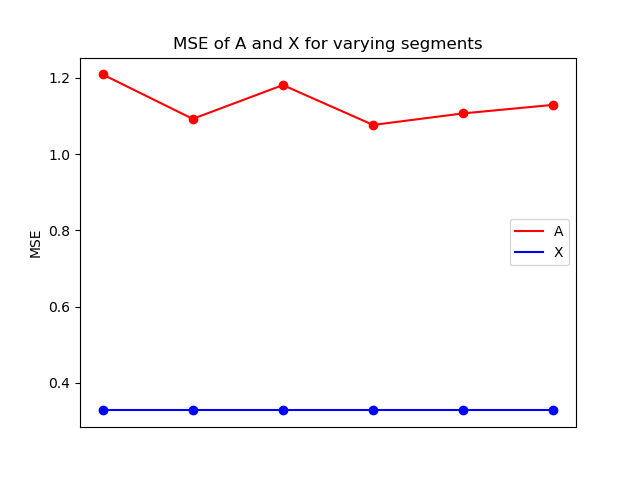
\includegraphics[scale=0.5]{figures/chapter6/Mix_Error_vary_covseg_m8_k16_L1000_RealA.png}
		\subcaption{Simple Data Set - Real A}
    \end{minipage} 
    \hfill
    \begin{minipage}[t]{.45\textwidth}
        \centering
		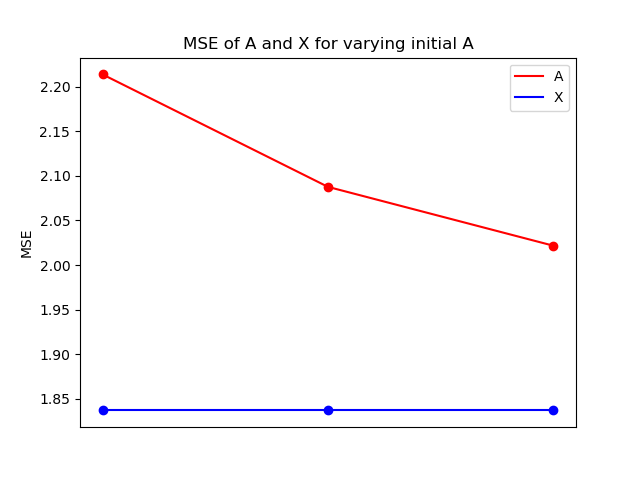
\includegraphics[scale=0.5]{figures/chapter6/AR_Error_initial_A_m8_k16_L1000_RealA.png}
		\subcaption{Autoregressive Data Set - Real A}
    \end{minipage}
\caption{}
\label{fig:seg}
\end{figure}
\noindent



\begin{table}[H]
\centering
\begin{minipage}{.5\linewidth}
\centering
\begin{tabular}{|c|c|c|c|c|c|c|}
\hline 
 & 10 & 20 & 30 & 40 & 50 & 60 \\ 
\hline 
MSE of $\mathbf{A}$ & 1.21 & 1.09 & 1.18 & 1.08 & 1.11 & 1.13 \\ 
\hline 
MSE of $\mathbf{X}$ & 0.69 & 0.64 & 0.68 & 0.64 & 0.65 & 0.64 \\ 
\hline 
\end{tabular} 
\subcaption{Simple Data Set - estimated $\mathbf{A}$}
\end{minipage}
\\
\begin{minipage}{.5\linewidth}
\centering
\begin{tabular}{|c|c|c|c|c|c|c|}
\hline 
 & 10 & 20 & 30 & 40 & 50 & 60 \\ 
\hline 
MSE of $\mathbf{A}$ & $\times$ & $\times$ & $\times$ & $\times$ & $\times$ & $\times$ \\ 
\hline 
MSE of $\mathbf{X}$ & 0.33 & 0.33 & 0.33 & 0.33 & 0.33 & 0.33 \\ 
\hline 
\end{tabular} 
\subcaption{Simple Data Set - real $\mathbf{A}$}
\end{minipage}
\\
\begin{minipage}{.5\linewidth}
\centering
\begin{tabular}{|c|c|c|c|c|c|c|}
\hline 
 & 10 & 20 & 30 & 40 & 50 & 60 \\ 
\hline
MSE of $\mathbf{A}$ & 1.87 & 1.90 & 1.70 & 1.92 & 1.85 & 1.88 \\
\hline 
MSE of $\mathbf{X}$ & 7.61 & 8.06 & 8.34 & 8.28 & 8.12 & 7.23 \\ 
\hline
\end{tabular} 
\subcaption{Autoregressive Data Set - estimated $\mathbf{A}$}
\end{minipage}
\\
\begin{minipage}{.5\linewidth}
\centering
\begin{tabular}{|c|c|c|c|c|c|c|}
\hline 
 & 10 & 20 & 30 & 40 & 50 & 60 \\ 
\hline 
MSE of $\mathbf{A}$ & $\times$ & $\times$ & $\times$ & $\times$ & $\times$ & $\times$ \\ 
\hline 
MSE of $\mathbf{X}$ & 2.15 & 2.15 & 2.15 & 2.15 & 2.15 & 2.15 \\  
\hline
\end{tabular} 
\subcaption{Autoregressive Data Set - real $\mathbf{A}$}
\end{minipage}
\caption{(a) This are the MSE values achieve from the simple data set and (b) is the MSE values achieved from the autoregressive data set.}
\label{tab:seg}
\end{table}
\noindent
